%*******************************************************************************
%*********************************** First Chapter *****************************
%*******************************************************************************

\chapter{Aplicaciones bioinformáticas para el estudio de interacciones miARN-gen blanco en plantas} 

\ifpdf
    \graphicspath{{Chapter1/Figs/Raster/}{Chapter1/Figs/PDF/}{Chapter1/Figs/}}
\else
    \graphicspath{{Chapter1/Figs/Vector/}{Chapter1/Figs/}}
\fi



\section{Introducción}


\section{Resultados} 

\subsection{Predicción de genes regulados por microARNs.} %Section - 1.1 
\subsubsection{Diseño de una estrategia para la identificación de genes blanco regulados por microARNs basado en la conservación evolutiva del par microARN-gen blanco.}

Enfocamos nuestro análisis en 22 miARNs que están conservados en Angiospermas (\citep{citeulike:8816489}, \citep{10.1371/journal.pgen.1002419}).  En general estos miARNs están codificados por pequeñas familias hasta 32 miembros. En los genomas completos de Arabidopsis, poplar y arroz es común encontrar variaciones en la secuencia de los miARNs pertenecientes a una misma familia, especialmente en el primer nucleótido y los nucleótidos 20 y 21 (\citep{10.1371/journal.pgen.1002419}).

Sin embargo, observamos que la región entre la posición 2 y 19 está bastante conservada y pudimos encontrar una secuencia consenso presente en la mayoría de los miembros de cada familia de miARNs en esas tres especies. (tabla \ref{table:table_consensus} y  tabla \ref{table:nice_table}).
Curiosamente, las bases variables fuera de esta región conservada son propensas a tener mismatches con genes blanco conocidos, lo que indica que podría existir una correlación entre la interacción miARN-gen blanco y la conservación de la secuencia del miARN.

Diseñamos una estrategia para identificar nuevos pares miARN-gen blanco principalmente basada en la conservación evolutiva de la secuencia del gen blanco (Figura \ref{fig:NAR_strategy}).
Las secuencias consenso de 18 nt de cada familia de miARN fueron usadas inicialmente para realizar la búsqueda de genes blanco en contigs de ESTs, de 41 especies de plantas, obtenidos de “Gene Index Project”\footnote{http://compbio.dfci.harvard.edu/tgi/} un proyecto mantenido y administrado por la universidad de Harvard que contiene un catálogo completo de genes en una amplia gama de organismos incluyendo plantas.
Además se utilizaron ARNm completos para \textit{A. thaliana}\footnote{http://arabidopsis.org} y \textit{Oryza Sativa}\footnote{http://rice.plantbiology.msu.edu} (para ver la lista completa de especies, ver tabla \ref{table:NAR_table_S2}).
Utilizando las secuencias consenso de 18nt y permitiendo 3 mismatches (errores), la búsqueda de genes blanco arrojó como resultado 38.597 genes distribuídos en las 43 especies (Figura \ref{fig:NAR_strategy}, bin 1).
Las interacciones G-U y los bulges fueron considerados como mismatches en esta primera búsqueda. Todos los genes blanco de  \textit{A. thaliana} conocidos hasta ese momento fueron identificados usando esta estrategia con la excepción de CSD2, un gen blanco del miR398 que contiene 4 mismatches ( tabla \ref{table:NAR_table_S2}).

Teniendo en cuenta que la mayoría de los genes blanco arrojados presentan una escasa descripción del tipo genómica funcional, realizamos un BLASTx  contra el proteoma de \textit{A. thaliana}.
El “locus ID” obtenido como “best hit” se utilizó como tag (etiqueta) para identificar al candidato en distintas especies (Figura \ref{fig:NAR_strategy}).
A pesar que esta estrategia no necesariamente identifica el gen ortólogo de Arabidopsis, sirve como propósito de clasificación de cada potencial gen blanco de miARN.
Aunque la mayoría de los potenciales genes blanco pudieron ser fácilmente asignados con una etiqueta, algunos pocos casos, que incluye a los genes que representan ARNs no codificantes fueron perdidos en este paso.

La estrategia permite la selección de los mejores candidatos basándose en la presencia de los genes blanco en un número distinto de especies.
Utilizando 4 especies como el mínimo de especies requeridas (ya que tiene una buena especificidad), dio como resultado 3.781 genes que corresponden a 533 tags diferentes (Figura \ref{fig:NAR_strategy}, bin 2).

La búsqueda también se puede hacer en combinación con filtros empíricos de interacción par miARN-gen blanco que tienen en cuenta la energía de interacción y la posición de los mismatches (ver Materiales y métodos).
De los 38.597 candidatos iniciales, 9.375 pasan estos filtros (Figura \ref{fig:NAR_strategy}, bin 4).
Combinando filtros de energía y filtro de conservación evolutiva, la búsqueda arrojó como resultado 563 candidatos correspondientes a 146 tags (Figura \ref{fig:NAR_strategy}, bin 5).


\begin{figure}[htbp!] 
    \centering    
    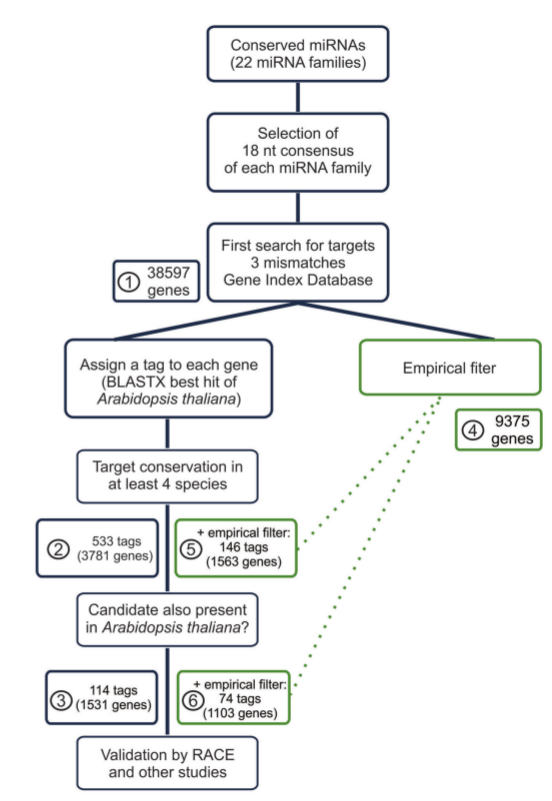
\includegraphics[width=0.7\textwidth]{strategy.png}
    \caption[Strategy]{Scheme of the strategy to identify new miRNA targets. The
number of detected target genes is indicated for each step of the
analysis. After applying the conservation analysis, all genes with
the same hit in the Arabidopsis proteome were considered as one
target. Note that different genes with the same ID tag give only one
hit, so that the total numbers of hits are reduced by this filter. Green
squares refer to the target search using empirical filters: bins 5 and 6
include target genes selected by both evolutionary and empirical filters,
while bins 2 and 3 have potential targets selected only by evolutionary
filters.
}
    \label{fig:NAR_strategy}
\end{figure}



\begin{table}
\tiny
\centering
\caption{miARNs y sus genes blancos en plantas}
\label{table:table_consensus}
\begin{tabular}{lllll}
\hline
\textbf{miARN} & \textbf{Consenso (18 nt)} & \textbf{Targets conocidos$^{(a,b)}$} &  &  \\ \hline
miR156 & GACAGAAGAGAGTGAGCA & factores de transcripción SPL&  &  \\
miR159 & TTGGATTGAAGGGAGCTC & factores de transcripción MYB, \textbf{NOZZLE (NZL)}&  &  \\
miR160 & GCCTGGCTCCCTGTATGC & factores de transcripción ARF&  &  \\
miR162 & CGATAAACCTCTGCATCC & DCL1&  &  \\
miR164 & GGAGAAGCAGGGCACGTG & factores de transcripción NAC&  &  \\
miR166 & CGGACCAGGCTTCATTCC & factores de transcripción HDZip&  &  \\
miR167 & GAAGCTGCCAGCATGATC & factores de transcripción ARF, \textbf{IAA-ALANINE RESISTANT 3 (IAR3)}&  &  \\
miR168 & CGCTTGGTGCAGGTCGGG & AGO1&  &  \\
mir169 & AGCCAAGGATGACTTGCC & factores de transcripción CCAAT-HAP2&  &  \\
mir171 & TTGAGCCGTGCCAATATC & factores de transcripción GRAS&  &  \\
miR172 & GAATCTTGATGATGCTGC & factores de transcripción AP2&  &  \\
miR319 & TGGACTGAAGGGAGCTCC & factores de transcripción TCP&  &  \\
miR390 & AGCTCAGGAGGGATAGCG & TAS RNA&  &  \\
miR393 & CCAAAGGGATCGCATTGA & TIR1 proteins, F-BOX proteins&  &  \\
miR394 & TGGCATTCTGTCCACCTC & proteínas F-BOX &  &  \\
miR395 & TGAAGTGTTTGGGGGAAC & ATP-sulfurilasas, transportadores de sulfato&  &  \\
miR396 & TCCACAGCTTTCTTGAAC & factores de transcripción GRF, \textbf{MMG4.7, FLUORESCENT IN BLUE LIGHT (FLU)}&  &  \\
miR397 & CATTGAGTGCAGCGTTGA & Laccases&  &  \\
miR398 & GTGTTCTCAGGTCACCCC & Cu/Zn SODs, CytC oxidase protein subunit, Chaperona de cobre (CCS)&  &  \\
miR399 & GCCAAAGGAGATTTGCCC & Enzima E2 de conjugación de ubiquitina&  &  \\
miR408 & TGCACTGCCTCTTCCCTG & Blue copper proteins, Laccases, \textbf{P-TYPE ATPase (PAA2), PAC1 (Proteasome component)}&  &  \\
miR827 & TAGATGACCATCAGCAAA & SPX proteins&  &  \\ \hline
\multicolumn{3}{l}{a Los genes blancos fueron agrupados según sus funciones.}\\
\multicolumn{3}{l}{b Nuevos genes blancos validados experimentalmente en este estudio están indicados en negrita.}\\

\end{tabular}
\end{table}

\subsubsection{Parámetros empíricos y de conservación evolutiva pueden actuar de manera sinérgica para identificar genes blanco regulados por miARNs.}
Potenciales genes blanco de miARNs fueron clasificados de acuerdo al mínimo número de especie en donde fueron detectados (Figura 2A-E).
Como control para cada microARN generamos 10 secuencias “scramble” (al azar), dividiendo las secuencias originales de a di-nucleótidos y luego generando nuevas secuencias al azar conservando la composición de los di-nucleótidos.
Estas secuencias al azar fueron utilizadas para realizar búsqueda de genes blanco del mismo modo que lo hicimos para las secuencias originales.
La relación señal/ruido fue calculada como el cociente entre el número de genes blanco para los miARNs y el número promedio obtenido de las secuencias al azar.
El radio fue de 1,2 para todos los miARNs juntos sin requerir conservación y esa relación incrementa con el número de especie en donde los genes blanco fueron detectados (Figura \ref{fig:NAR_fig2} A, recuadro). 
Los datos para todos los miARNs y sus potenciales genes blancos conservados en al menos 4 especies están incluidos en la tabla \ref{table:NAR_table_2}.

Luego estudiamos la selección de candidatos teniendo en cuenta los filtros empíricos.
Para esto aplicamos una versión modificada de los filtros descritos anteriormente y requiriendo (i) una energía mínima de hibridación (MFE) de al menos 72\% del apareamiento perfecto de cada secuencia consenso y (ii) que sólo un mismatch pudiera estar presente entre la posición 1 y la 11 de la secuencia consenso (2-12 del miARN).
De la búsqueda inicial 9.375 genes pasaron estos filtros conteniendo el 97\% de los genes validados anteriormente de Arabidopsis. (Figura \ref{fig:NAR_strategy}, bin 4). 

Al aplicar solamente este filtro empírico, dio como resultado una relación señal/ruido de 1,7, al agrupar todos los miARNs juntos (Figura \ref{fig:NAR_fig2} A).
Observamos que aplicar simultáneamente los filtros empíricos y de conservación aumentaron significativamente la relación señal/ruido para todos los miARNs juntos (Figura \ref{fig:NAR_fig2} A recuadro) y también de cada miARN individualmente (Figura \ref{fig:NAR_fig2} B-E, recuadros y tabla \ref{table:NAR_table_2}).
En varios casos, esta relación llega hasta 10 cuando se requiere de que el gen blanco este presente en más de 5 especies y que pase los filtros empíricos (Figure \ref{fig:NAR_fig2} A–D).
Este efecto sinérgico indica que el filtro de conservación evolutiva y los parámetros empíricos pueden estar seleccionando aspectos diferentes de la interacción miARN-gen blanco.

Observamos que el número de genes blanco candidato y la relación señal/ruido es variable entre los distintos miARNs.
El miR396 tiene la mayor cantidad de potenciales genes blanco, 92 de ellos presentes en al menos 4 especies y 26 de ellos pasan además los filtros empíricos (Tabla \ref{table:NAR_table_2} y Figura \ref{fig:NAR_fig2} B).
El miR408 y el miR398 también tienen un número alto de potenciales genes blanco y buenas relaciones de señal/ruido (Figura \ref{fig:NAR_fig2} C-D).

En contraste, ciertos miARNs como el miR162, miR168 y miR399 tienen un solo potencial gen blanco conservado en al menos 4 especies de acuerdo con nuestra búsqueda ( Tabla \ref{table:NAR_table_2} y Figura \ref{fig:NAR_fig2} E).
Al menos en el caso del miR162 y del miR168 este resultado podría estar reflejando su rol específico en la regulación por retroalimentación de la biogénesis del miARN, ya que controlan los niveles de expresión DCL1 y AGO1 respectivamente (\citep{Vazquez2004},\citep{Xie2003}).

Como control adicional para nuestra estrategia hicimos la búsqueda de genes blanco del miR158 y miR173, que son miARNs presentes solamente en A. thaliana y especies bien cercanas (17). Como era esperado estos miARNs no generaron más candidatos que sus versiones al azar (Tabla \ref{table:NAR_table_2} y Figura \ref{fig:NAR_fig2} F).


Luego chequeamos si los pares miARN-gen blanco altamente conservados tenían una interacción más fuerte que los que están presentes en pocas especies.
Para esto calculamos la energía mínima de hibridación para cada interacción detectada en nuestro trabajo. 
Observamos que los pares miARN-gen blanco presentes en muchas especies tienden a tener energía de interacción mayores que los que están presentes en menos especies (Figure \ref{fig:NAR_fig3} A).
De todos modos, la correlación no fue notoria y algunas interacciones miARN-gen blanco tuvieron una baja energía de hibridación (Figure \ref{fig:NAR_fig3} A).
Estos resultados muestran que una alta conservación podría no ser necesariamente equivalente a una fuerte interacción, la misma podría proporcionar una explicación para los efectos sinérgicos causados por los filtros de evolución y empíricos sobre la relación señal/ruido.

\begin{figure}[htbp!] 
    \centering    
    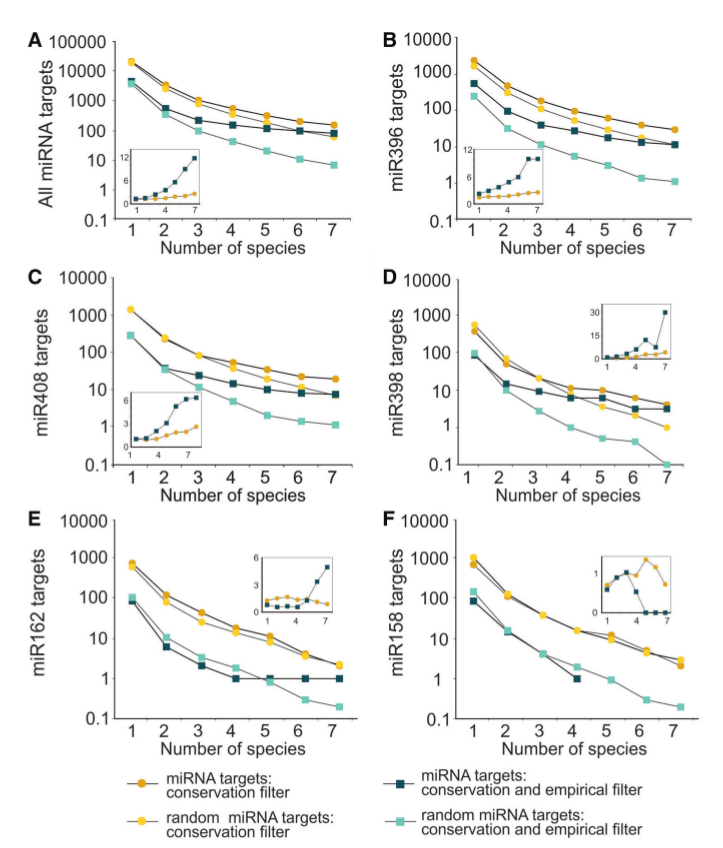
\includegraphics[width=0.7\textwidth]{NAR_fig2.png}
    \caption[]{Conservación de potenciales genes blanco en distintas especies. Todos los miARNs (A), miR396 (B), miR408 (C), miR398 (D), miR162 (E), miR158 (F). Puntos naranja representan los genes blanco de miARNs usando filtro evolutivo. Puntos amarillos representan los genes blanco de las secuencias al azar usando filtro evolutivo. El cuadrado azul muestra los genes blanco de miARNs luego de aplicar filtros empíricos y evolutivos, mientras que el cuadrado celeste representa los genes blanco de las secuencias al azar en las mismas condiciones. Los recuadros muestran la relación señal/ruido.}
    \label{fig:NAR_fig2}
\end{figure}

\begin{figure}[htbp!] 
    \centering    
    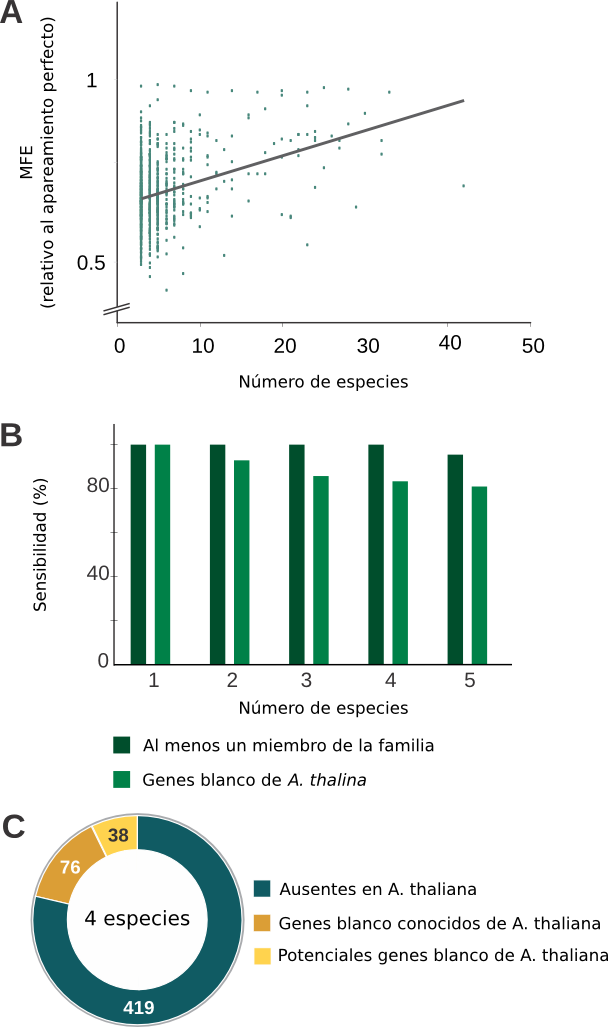
\includegraphics[width=0.7\textwidth]{NAR_fig3.png}
    \caption[]{Selección de genes blanco por conservación evolutiva de la secuencia. (A) Relación entre MFE y el número de especies en donde cada gen blanco fue detectado. (B) Sensibilidad de la estrategia, analizado de dos modos distinto. Verde clarito: evaluando la presencia de genes validados en Arabidopsis y en verde oscuro teniendo en cuenta la presencia de por lo menos un gen blanco de cada familia regulada por miARNs. (C) Clasificación de los potenciales genes blanco presentes en al menos 4 especies.}
    \label{fig:NAR_fig3}
\end{figure}





\begin{landscape}
\begin{table}[]
\tiny
\centering
\caption{Detection of miRNA targets using different filters}
\label{table:NAR_table_2}
\begin{tabular}{lllllllllllllllll}
\multicolumn{1}{c}{} & \multicolumn{4}{c}{\textbf{Sin filtros}}                        & \multicolumn{4}{c}{\textbf{Filtros empíricos}}                  & \multicolumn{4}{c}{\textbf{Conservación 4 especies}}            & \multicolumn{4}{c}{\textbf{Todos los filtros}}                  \\
\multicolumn{1}{c}{} & \multicolumn{1}{c}{\textbf{miARN}} & \multicolumn{1}{c}{\textbf{scramble}} & \multicolumn{1}{c}{\textbf{}} & \multicolumn{1}{c}{\textbf{ratio}} & \multicolumn{1}{c}{\textbf{miARN}} & \multicolumn{1}{c}{\textbf{scramble}} & \multicolumn{1}{c}{\textbf{}} & \multicolumn{1}{c}{\textbf{ratio}} & \multicolumn{1}{c}{\textbf{miARN}} & \multicolumn{1}{c}{\textbf{scramble}} & \multicolumn{1}{c}{\textbf{}} & \multicolumn{1}{c}{\textbf{ratio}} & \multicolumn{1}{c}{\textbf{miARN}} & \multicolumn{1}{c}{\textbf{scramble}} & \multicolumn{1}{c}{\textbf{}} & \multicolumn{1}{c}{\textbf{ratio}} \\
\textbf{miR156}      & 3915           & 3994.4            & $\pm$ 149.9     & 1.0            & 890            & 704.7             & $\pm$  45.2      & 1.3            & 34             & 39.7              & $\pm$  3.1       & 0.9            & 10             & 5.4               & $\pm$  1.1       & 1.9            \\
\textbf{miR159}      & 1663           & 1283.7            & $\pm$  47.8      & 1.3            & 472            & 254.9             & $\pm$  21.9      & 1.9            & 20             & 10.1              & $\pm$  1.1       & 2.0            & 6              & 1.5               & $\pm$  0.5       & 4.0            \\
\textbf{miR160}      & 793            & 695.6             & $\pm$  30.5      & 1.1            & 277            & 157.5             & $\pm$  28.8      & 1.8            & 5              & 4.4               & $\pm$  0.9       & 1.1            & 4              & 0.5               & $\pm$  0.3       & 8.0            \\
\textbf{miR162}      & 1191           & 930.2             & $\pm$  139.5     & 1.3            & 108            & 164.7             & $\pm$  24.1      & 0.7            & 18             & 13.5              & $\pm$  3.5       & 1.3            & 1              & 1.8               &  $\pm$ 0.5       & 0.6            \\
\textbf{miR164}      & 2486           & 1480.2            & $\pm$  60.4      & 1.7            & 678            & 333.2             & $\pm$  32.2      & 2.0            & 39             & 12.4              & $\pm$  1.9       & 3.1            & 12             & 1.5               & $\pm$  0.5       & 8.0            \\
\textbf{miR166}      & 879            & 815.5             & $\pm$  45.0      & 1.1            & 231            & 129               & $\pm$  14.5      & 1.8            & 16             & 10.6              & $\pm$  1.4       & 1.5            & 6              & 0.9               & $\pm$  0.4       & 6.7            \\
\textbf{miR167}      & 1777           & 1364.2            & $\pm$  146.6     & 1.3            & 478            & 214.8             & $\pm$  27.5      & 2.2            & 22             & 20.2              & $\pm$  3.6       & 1.1            & 4              & 1.8               & $\pm$  0.5       & 2.2            \\
\textbf{miR168}      & 962            & 797.5             & $\pm$  48.5      & 1.2            & 209            & 185               & $\pm$  14.2      & 1.1            & 6              & 4.4               & $\pm$  0.8       & 1.4            & 1              & 1.1               & $\pm$  0.5       & 0.9            \\
\textbf{miR169}      & 1540           & 1047.2            & $\pm$  69.7      & 1.5            & 464            & 181.4             & $\pm$  15.6      & 2.6            & 26             & 11.1              & $\pm$  2.1       & 2.3            & 10             & 1.2               & $\pm$  0.2       & 8.3            \\
\textbf{miR171}      & 884            & 723.4             & $\pm$  32.1      & 1.2            & 202            & 113.8             & $\pm$  13.4      & 1.8            & 7              & 6.6               & $\pm$  1.4       & 1.1            & 2              & 0.7               & $\pm$  0.3       & 2.9            \\
\textbf{miR172}      & 3007           & 1693.7            & $\pm$  124.7     & 1.8            & 540            & 288.1             & $\pm$  40.3      & 1.9            & 34             & 17.7              & $\pm$  1.7       & 1.9            & 5              & 2.2               & $\pm$  0.6       & 2.3            \\
\textbf{miR319}      & 1363           & 1274.2            & $\pm$  113.6     & 1.1            & 324            & 249.2             & $\pm$  22.3      & 1.3            & 18             & 15                & $\pm$  2.8       & 1.2            & 7              & 1.8               & $\pm$  0.5       & 3.9            \\
\textbf{miR390}      & 873            & 814.4             & $\pm$  64.3      & 1.1            & 335            & 173               & $\pm$  22.5      & 1.9            & 8              & 4.7               & $\pm$  1.2       & 1.7            & 3              & 0.7               & $\pm$  0.5       & 4.3            \\
\textbf{miR393}      & 986            & 844.6             & $\pm$  58.7      & 1.2            & 276            & 124.6             & $\pm$  11.1      & 2.2            & 14             & 7.1               & $\pm$  1.2       & 2.0            & 5              & 0.5               & $\pm$  0.2       & 10.0           \\
\textbf{miR394}      & 1569           & 1531.4            & $\pm$  57.5      & 1.0            & 188            & 237.1             & $\pm$  25.0      & 0.8            & 26             & 21.4              & $\pm$  2.2       & 1.2            & 3              & 2.9               & $\pm$  0.5       & 1.0            \\
\textbf{miR395}      & 1472           & 1226.7            & $\pm$  66.7      & 1.2            & 426            & 217.6             & $\pm$  16.5      & 2.0            & 11             & 8.8               & $\pm$  1.3       & 1.3            & 6              & 1.3               & $\pm$  0.3       & 4.6            \\
\textbf{miR396}      & 4641           & 2979.3            & $\pm$  246.6     & 1.6            & 1246           & 390.5             & $\pm$  38.8      & 3.2            & 92             & 51.4              & $\pm$  5.9       & 1.8            & 26             & 5.4               & $\pm$  1.0       & 4.8            \\
\textbf{miR397}      & 1426           & 1050.9            & $\pm$  27.9      & 1.4            & 368            & 236.5             & $\pm$  23.5      & 1.6            & 26             & 9.7               & $\pm$  0.8       & 2.7            & 10             & 1.6               & $\pm$  0.3       & 6.3            \\
\textbf{miR398}      & 935            & 834               & $\pm$  34.5      & 1.1            & 376            & 144               & $\pm$  18.1      & 2.6            & 11             & 7.5               & $\pm$  1.6       & 1.5            & 6              & 1                 & $\pm$  0.3       & 6.0            \\
\textbf{miR399}      & 1192           & 1137.6            & $\pm$  72.0      & 1.0            & 275            & 207.8             & $\pm$  24.9      & 1.3            & 5              & 13.6              & $\pm$  1.7       & 0.4            & 1              & 1.5               & $\pm$  0.7       & 0.7            \\
\textbf{miR408}      & 2782           & 2502.9            & $\pm$  103.6     & 1.1            & 695            & 468.7             & $\pm$  50.8      & 1.5            & 51             & 35.1              & $\pm$  3.0       & 1.5            & 14             & 4.6               & $\pm$  0.8       & 3.0            \\
\textbf{miR827}      & 2261           & 2000.1            & $\pm$  119.8     & 1.1            & 317            & 297.1             & $\pm$  45.0      & 1.1            & 44             & 23.4              & $\pm$  3.9       & 1.9            & 4              & 2.3               & $\pm$  0.8       & 1.7            \\
\textbf{Total}       & 38597          & 31021.7           & $\pm$  1859.8    & 1.2            & 9375           & 5473.2            & $\pm$  576.3     & 1.7            & 533            & 348.4             & $\pm$  47.0      & 1.5            & 146            & 42.2              & $\pm$  11.3      & 3.5            \\
\textbf{Control}     &                &                   &                  &                &                &                   & $\pm$            &                &                &                   &                  &                &                &                   &                  &                \\
\textbf{miR158}      & 1364           & 1462.8            & $\pm$  69.1      & 0.9            & 170            & 208.7             & $\pm$  15.8      & 0.8            & 15             & 16                & $\pm$  1.7       & 0.9            & 1              & 1.9               & $\pm$  0.4       & 0.5            \\
\textbf{miR173}      & 1386           & 1232.1            & $\pm$  101.7     & 1.1            & 243            & 215.6             & $\pm$  23.4      & 1.1            & 11             & 12                & $\pm$  2.4       & 0.9            & 1              & 1.5               & $\pm$  0.4       & 0.7           \\
\multicolumn{17}{l}{a Sin filtros, búsqueda inicial utilizando los miARN consenso de 18nt y 3 mismatches.}\\
\multicolumn{17}{l}{b Filtros empíricos, energía de al menos 72\% del apareamiento perfecto y 1 mismatch en la posición 2-12 del par miARN-gen blanco.}\\
\multicolumn{17}{l}{c Conservación del ID tag en al menos cuatro especies.}\\
\multicolumn{17}{l}{d Todos los filtros, combinación de los filtros empíricos y de conservación en al menos cuatro especies.}\\
\multicolumn{17}{l}{e miARN, genes blanco para cada miARN específico.}\\
\multicolumn{17}{l}{f scramble, promedio de los genes blanco de 10 versiones al azar de cada miARN ± error estándar.}\\
\end{tabular}
\end{table}
\end{landscape}

\subsubsection{Identificación de nuevos genes blanco en \textit{A. thaliana} por conservación de la secuencia del gen blanco.}
\subsubsection{Identificación de nuevos genes blanco permitiendo interacciones G-U.}
\subsubsection{Identificación de genes blanco específicos de \textit{Solanaceae}.}

\subsection{comTAR: una herramienta para la predicción de genes blanco regulados por microARNs en plantas.} 

\subsection{Where does it come from?}  

